\section{性能追踪系统}
\label{sec:perfetto}

\subsection{背景}

游戏引擎性能优化需要精确的性能数据。开发者需要了解：哪个函数消耗了最多时间？哪个线程是瓶颈？帧时间花在哪里？传统的日志和手动计时方法存在以下问题：

\begin{enumerate}
    \item \textbf{侵入性强}：需要手动插入计时代码，维护成本高
    \item \textbf{开销大}：频繁的时间戳获取影响测量结果
    \item \textbf{信息不足}：缺乏函数调用栈和线程时序信息
    \item \textbf{难以关联}：跨系统的事件难以追踪因果关系
\end{enumerate}

\subsection{原版局限性}

Java版Minecraft的性能分析依赖外部工具：

\begin{enumerate}
    \item \textbf{JProfiler、VisualVM等}：运行时开销可达10-20\%，影响测量准确性
    \item \textbf{手动计时代码}：分散在代码各处，容易遗漏或过时
    \item \textbf{缺乏细粒度帧内分析}：无法详细了解单帧内的时间分布
    \item \textbf{无法关联跨系统事件}：例如，无法追踪方块设置到光照更新到网格重建的完整链路
\end{enumerate}

\subsection{本项目实现}

本项目集成Perfetto性能追踪SDK，实现低开销、高精度的性能观测。整体架构如图\ref{fig:perfetto_arch}所示。

\begin{figure}[h]
\centering
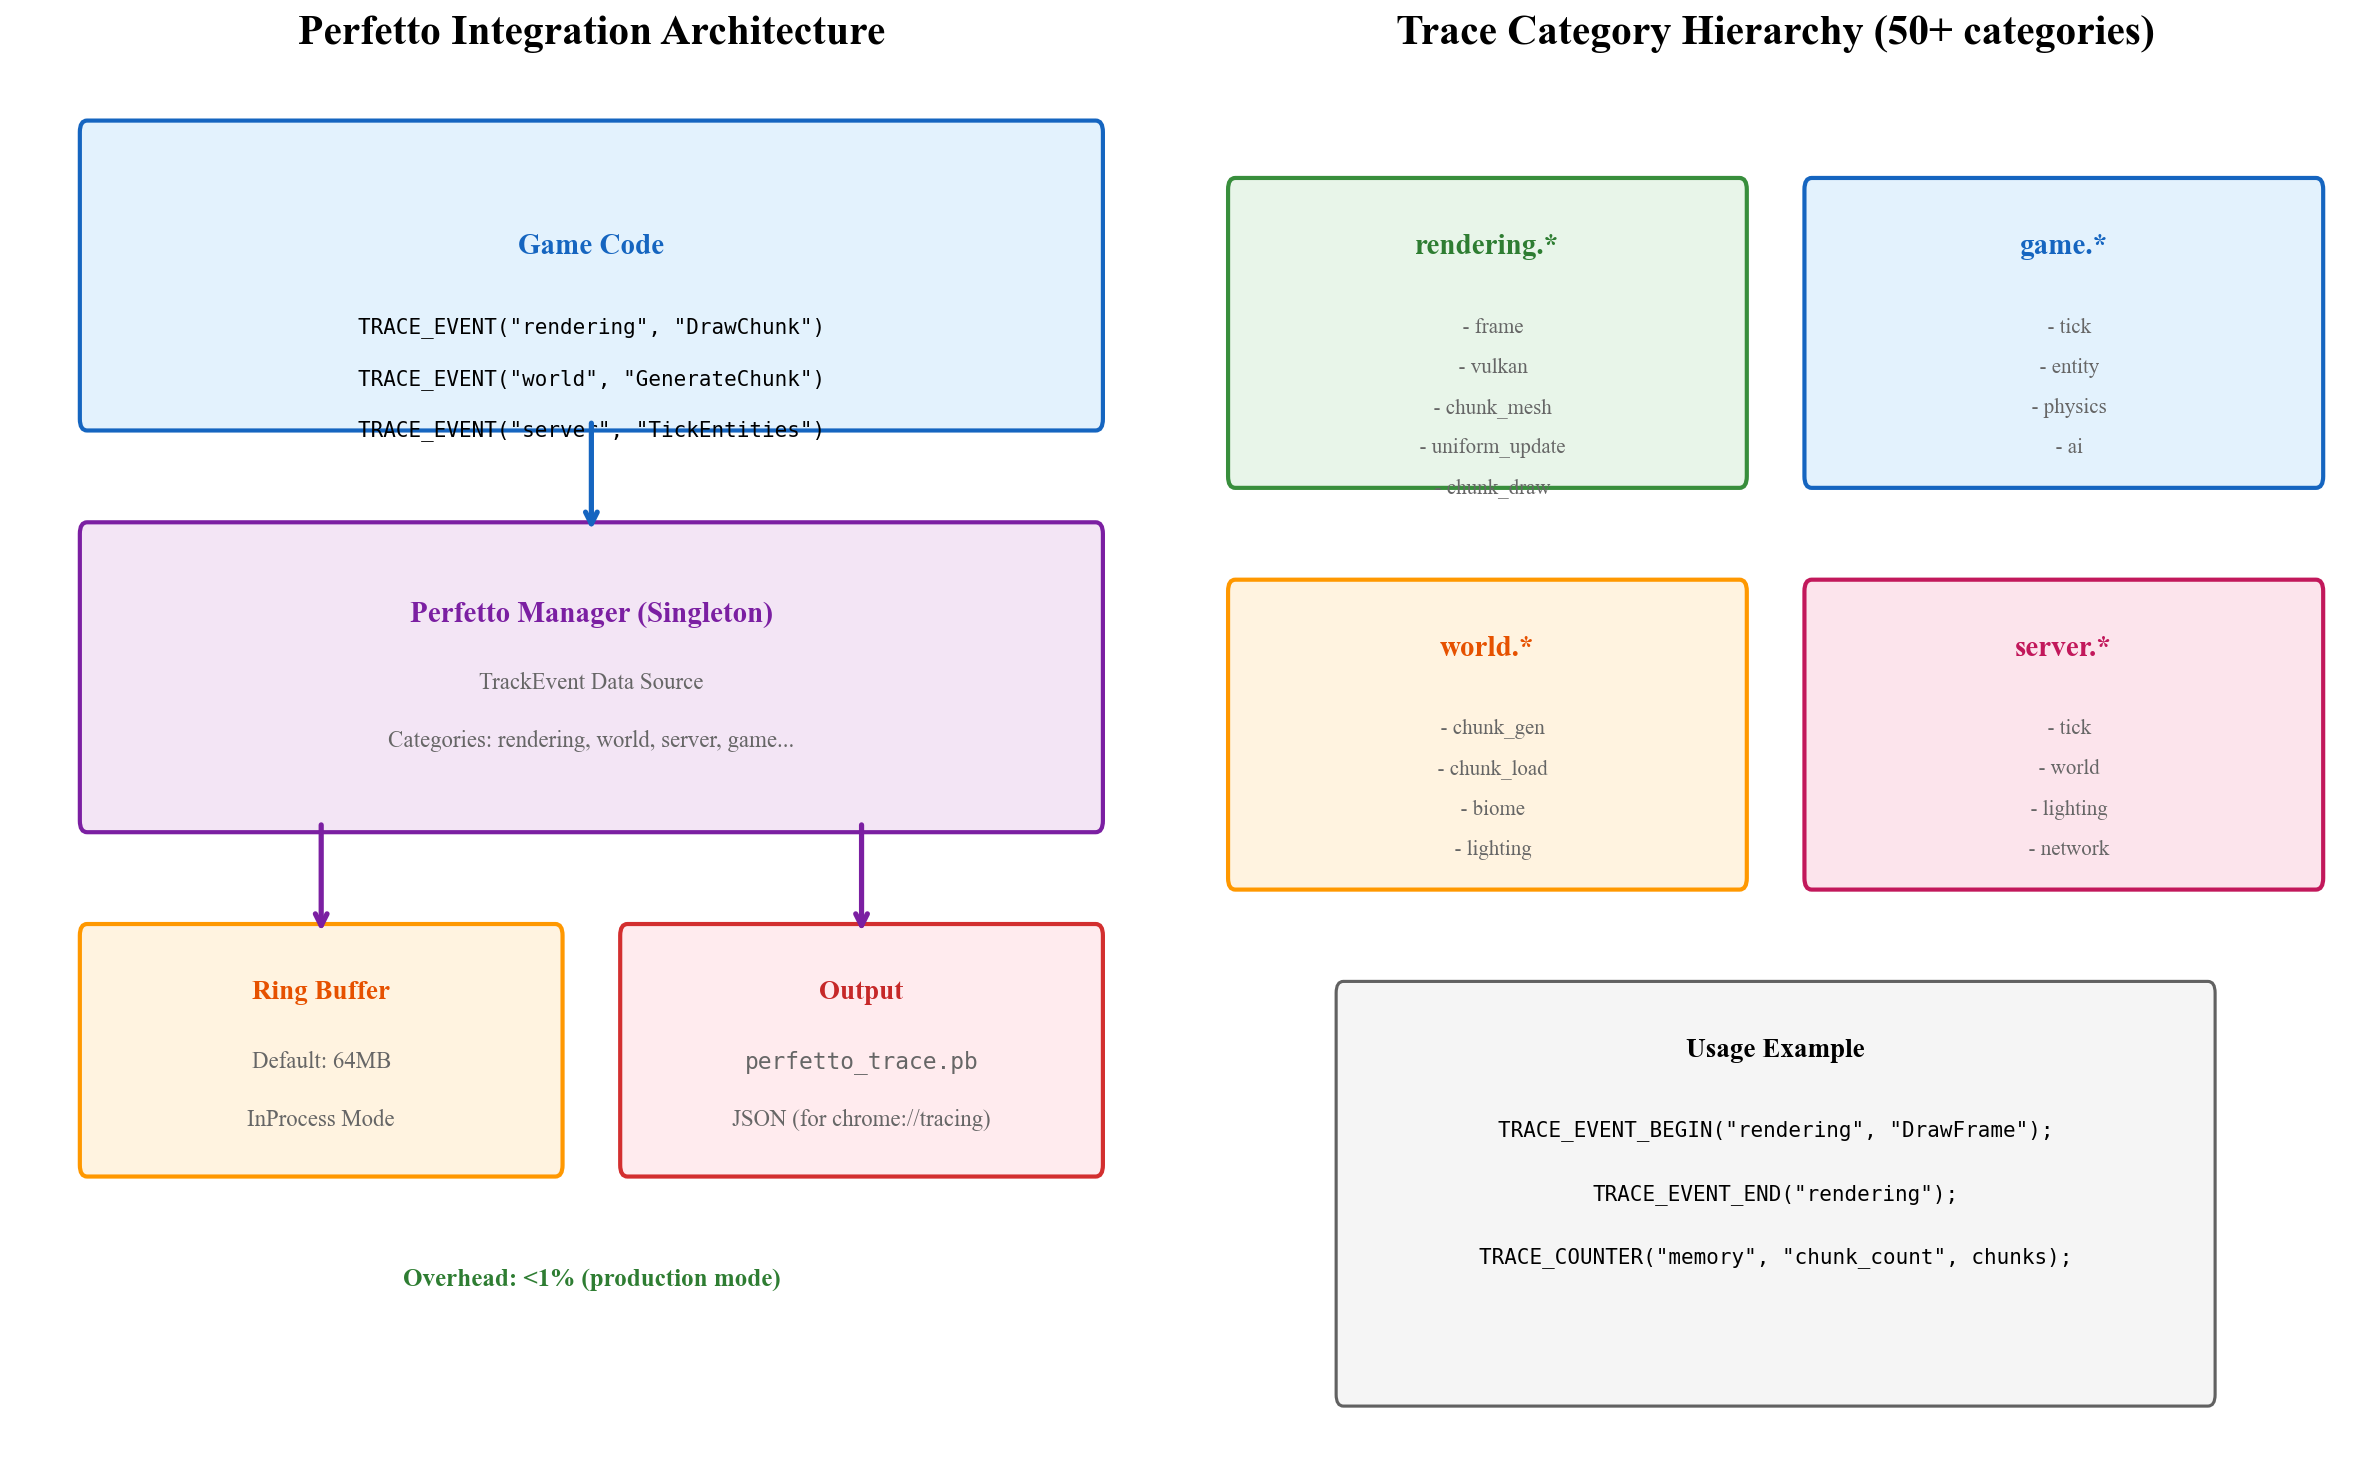
\includegraphics[width=0.95\linewidth]{images/perfetto_system.png}
\caption{Perfetto集成架构。左图展示追踪数据流：游戏代码通过TRACE\_EVENT宏记录事件，Perfetto管理器将数据写入环形缓冲区，最终输出为protobuf格式。右图展示50+追踪分类的层次结构。}
\label{fig:perfetto_arch}
\end{figure}

\subsubsection{架构设计}

Perfetto管理器采用单例模式，全局唯一实例管理追踪会话的生命周期：

\textbf{初始化流程}：
\begin{enumerate}
    \item 创建Perfetto实例，配置后端（InProcess模式）
    \item 注册TrackEvent数据源
    \item 创建追踪会话，配置缓冲区大小（默认64MB）
    \item 启动追踪
\end{enumerate}

\textbf{追踪配置}：支持启用/禁用特定分类、设置输出文件路径、配置缓冲区大小等。生产环境可以只启用关键分类，减少开销。

\subsubsection{追踪分类体系}

定义了50+个追踪分类，覆盖所有子系统：

\textbf{渲染相关}：
\begin{itemize}
    \item \texttt{rendering.frame}：帧渲染生命周期事件
    \item \texttt{rendering.vulkan}：Vulkan API调用
    \item \texttt{rendering.chunk\_mesh}：区块网格生成和上传
    \item \texttt{rendering.begin\_frame}：帧开始阶段（等待同步、获取图像）
    \item \texttt{rendering.uniform\_update}：Uniform缓冲区更新
    \item \texttt{rendering.chunk\_draw}：区块绘制（绑定管线、描述符、绘制调用）
\end{itemize}

\textbf{游戏逻辑相关}：
\begin{itemize}
    \item \texttt{game.tick}：游戏刻处理
    \item \texttt{game.entity}：实体更新
    \item \texttt{game.physics}：物理模拟
    \item \texttt{game.ai}：AI目标处理
\end{itemize}

\textbf{世界相关}：
\begin{itemize}
    \item \texttt{world.chunk\_gen}：区块生成各阶段
    \item \texttt{world.chunk\_load}：区块加载和卸载
    \item \texttt{world.biome}：生物群系生成
\end{itemize}

\textbf{服务端相关}：
\begin{itemize}
    \item \texttt{server.tick}：服务端游戏刻处理
    \item \texttt{server.world}：服务端世界更新
    \item \texttt{server.lighting}：服务端光照处理
    \item \texttt{server.network}：网络处理
\end{itemize}

\textbf{工作池相关}：
\begin{itemize}
    \item \texttt{worker\_pool}：通用任务池操作
    \item \texttt{worker\_pool.chunk\_gen}：区块生成任务
    \item \texttt{worker\_pool.chunk\_io}：区块IO任务
\end{itemize}

\subsubsection{追踪事件宏}

定义零开销的追踪宏，在编译时决定是否启用：

\textbf{作用域事件}：自动记录进入和退出时间，使用RAII模式。
\begin{equation}
T_{duration} = t_{exit} - t_{enter}
\end{equation}

\textbf{计数器事件}：记录数值随时间的变化，用于FPS、内存使用等指标追踪。

\textbf{Flow事件关联}：使用\texttt{Flow::ProcessScoped}关联跨系统事件。例如，设置方块事件可以关联到光照更新事件，再到网格重建事件，形成完整的因果链。

当\texttt{MC\_ENABLE\_TRACING}为0时，所有宏展开为空操作\texttt{((void)0)}，实现零性能开销。

\subsubsection{线程命名}

在工作线程入口设置线程名称，使得追踪结果中可以清晰地区分不同线程：
\begin{itemize}
    \item \texttt{ServerWorker-0}、\texttt{ServerWorker-1}等：服务端工作线程
    \item \texttt{ChunkMeshWorker-0}、\texttt{ChunkMeshWorker-1}等：客户端网格构建线程
    \item \texttt{ClientMainThread}：客户端主线程
\end{itemize}

\subsubsection{使用示例}

\textbf{帧渲染追踪}：在主循环中，使用作用域事件追踪帧渲染的各个阶段。每个阶段可以添加键值对参数，如\texttt{"phase", "handle\_events"}。

\textbf{方块设置追踪}：在\texttt{ServerWorld::setBlockState}中，记录坐标参数，并使用Flow关联后续的光照更新和网格重建事件。

\textbf{工作线程追踪}：在任务执行前后记录任务类型、描述和优先级，用于分析线程池利用率。

\textbf{性能计数器}：每帧记录FPS和内存使用，生成时间序列图表。

\subsection{解决与成果}

\begin{table}[h]
\centering
\caption{追踪覆盖范围}
\label{tab:trace_coverage}
\begin{tabular}{lcc}
\toprule
\textbf{子系统} & \textbf{追踪分类数} & \textbf{关键追踪点} \\
\midrule
渲染系统 & 15+ & 帧时间、Vulkan调用、网格构建 \\
游戏逻辑 & 5+ & Tick、实体更新、物理 \\
世界生成 & 5+ & 区块生成、加载、生物群系 \\
网络层 & 3+ & 数据包处理、同步 \\
服务端 & 6+ & Tick、世界更新、光照 \\
存储层 & 3+ & 读写、缓存命中 \\
\bottomrule
\end{tabular}
\end{table}

追踪数据输出为Perfetto二进制格式（\texttt{.perfetto-trace}文件），可通过\texttt{ui.perfetto.dev}进行分析：

\begin{itemize}
    \item \textbf{时间线视图}：按线程展示所有事件，直观看到时间分布
    \item \textbf{火焰图}：函数调用栈分析，识别热点函数
    \item \textbf{计数器图表}：FPS、内存等数值随时间变化
    \item \textbf{Flow关联}：追踪事件跨系统传播路径
\end{itemize}

禁用追踪时所有宏展开为空操作，实现零性能开销。启用追踪时，每个事件的overhead约为纳秒级别，对帧率影响可忽略。
